\subsection{The Proof-of-Stake Block}
In every slot (spaced twelve seconds apart) a validator is randomly selected to be the block proposer. They bundle transactions together, execute them and determine a new 'state'. They wrap this information into a \textbf{block} and pass it around to other validators.

\textbf{Other validators re-execute and validate}: Validators who hear about the new block re-execute the transactions to ensure they agree with the proposed change to the global state. Assuming the block is valid, they add it to their own database.

If a validator hears about two conflicting blocks for the same slot they use their fork-choice algorithm to pick the one supported by the most staked ETH.

\begin{wrapfigure}{r}{0.40\textwidth}
    \centering
    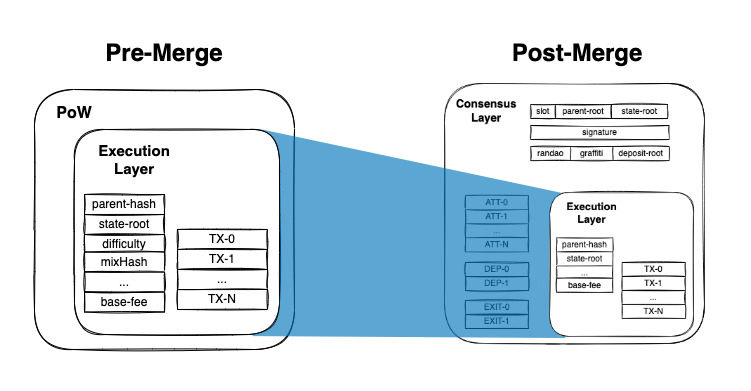
\includegraphics[width=0.40\textwidth]{ethereum/assets/block-merge.png}
    \caption{The Proof-of-Stake Block}
    \label{fig:pos-block}
\end{wrapfigure}

Previously, the Ethereum's Proof-of-Work Block (PoW Block) only contained execution related information. Post-Merge, the new Proof-of-Stake Block (PoS Block) will contain ACE information: 
\begin{itemize}
    \item \textbf{A}dministration (the metadata of the block)
    \item \textbf{C}onsensus (Beacon Chain co-ordination)
    \item \textbf{E}xecution (Block data)
\end{itemize}
This makes PoW Block more or less a subset of the new PoS Block. See \ref{fig:pos-block}.

